\documentclass[amsmath, amssymb]{revtex4}
% \documentclass[dvips,aoas,preprint]{imsart}
% \documentclass{article}

\usepackage{algorithm}
\usepackage{algpseudocode}
\usepackage{graphicx}% Include figure files
\usepackage{amsmath}
\usepackage{amsfonts}
\usepackage{amsthm}
\usepackage{charter}
%\usepackage{cite}
%\usepackage{algorithmic}

%\usepackage{dcolumn}% Align table columns on decimal point
%\usepackage{bm}% bold math
\RequirePackage[OT1]{fontenc}
\RequirePackage{amsthm,amsmath,natbib}
%\RequirePackage[colorlinks,citecolor=blue,urlcolor=blue]{hyperref}
% \RequirePackage{hypernat}

%\startlocaldefs
\renewcommand{\i}{\backslash i}
\newcommand{\bth}{\mathbf{\theta}}
\newcommand{\w}{w}
\newcommand{\bw}{\mathbf{\w}}
\newcommand{\T}{^{\ensuremath{\mathsf{T}}}}           % transpose
\DeclareMathOperator*{\argmax}{argmax}
\DeclareMathOperator*{\argmin}{argmin}
\newcommand{\bF}{{\bf F}}
\newcommand{\bX}{{\bf X}}
\newcommand{\bn}{{\bf n}}
\newcommand{\bh}{\mathbf{h}}
\newcommand{\hbth}{\widehat{\bth}}
\newcommand{\hbw}{\widehat{\bw}}
\newcommand{\sumit}{\sum_{\substack{i \in [1,\ldots,N] \\ t \in [1,\ldots, T]}}}
%\endlocaldefs


\begin{document}

%\author{}
% \altaffiliation[Also at ]{Physics Department, XYZ University.}
%\author{Second Author}%
% \email{Second.Author@institution.edu}
%\affiliation{%
%Authors' institution and/or address\\
%This line break forced with \textbackslash\textbackslash
%}%
%\author{Charlie Author}
% \homepage{http://www.Second.institution.edu/~Charlie.Author}
%\affiliation{
%Second institution and/or address\\
%This line break forced% with \\
%}%
%\preprint{APS/123-QED}
%\pacs{Valid PACS appear here}
%\keywords{Suggested keywords}

\date{\today}

\title{Bayesian inference of neural connectivity in a population of neurons from 
calcium imaging data}


\begin{abstract}
Simultaneously imaging small populations of neurons using calcium sensors is now becoming routine in labs across the world.  We have developed analytical tools to maximally utilize these beautiful data sets.  In particular, the following neurobiological questions are of interest: (i) what are the response properties of populations of neurons that are in close physical proximity, (ii) what is the functional circuit underlying these response properties.  Previously, we built a forward model characterizing the relationship between stimuli, spike trains, intracellular calcium concentration, and fluorescence time series observations; and then inverted that model using non-linear state-space methods (i.e., a particle-filter-smoother adapted for this model, embedded in an expectation-maximization algorithm).  

Here, that forward model is generalized to allow for dependencies between neurons (i.e., cross-coupling terms), and the inference and learning algorithm is appropriately modified as well.  We show that given only a short movie (< 10 min), and reasonable assumptions on noisiness, spike rates, and coupling strengths, we can accurately reconstruct circuits governing small populations (e.g., 10 neurons; see S1).  As the number of neurons increases, or the data quality decreases, we can impose experimentally justifiable priors on the distribution of coupling weights, to improve our estimates.  

We are currently pursuing confirming our parameter estimates using in vitro preparations.  In particular, by simultaneously imaging a population of neurons, and recording electrophysiologically from at least one, we can validate our inferred connection strengths.  Our hope is that they algorithms developed here will be useful in a wide array of experiments and preparations, especially in vivo calcium imaging.
\end{abstract}

\maketitle
\tableofcontents

\section{Motivation}
\label{intro}
Since Ramon y Cajal discovered that the brain is not a syncytium, but rather a rich and dense \emph{network} of neurons, neuroscientists have wondered about the details of these networks.  Since then, while much has been learned about ``macro-circuits''  --- the connectivity between populations of neurons --- relatively little is known about ``micro-circuits'' --- the connectivity within populations of neurons. Broadly, one can imagine two distinct strategies for inferring microcircuit connectivity: anatomical and functional.  

Anatomical approaches, while perhaps the gold standard for questions of connectivity, are often exceedingly laborious.  Historically, neuroanatomists used tracing studies to address these questions,  i.e., filled individual neurons with various dyes, and looked where the axons and dendrites terminated \cite{??}.  Besides being problematic with respect to whether the dyes filled the processes to the far proximal limit, or merely until the diameter became too small \cite{??}, this process is tedious and very low throughput.  Recently, experimentalists have developed fluorescent proteins that express throughout the dendritic tree \cite{??} or axonal arborization \cite{??}, that potentially resolves the premature termination issue, but not the throughput issue. Complementary to these labeling ideas, others have been developing Electron Microscopy based strategies to slice up neural tissue \cite{??}, and then automate track tracing using sophisticated image processing software \cite{??}.  This strategy has great promise for improving the throughput of these neuroanatomical studies, but have not yet quite achieved ``off-the-shelf'' status for experimental neuroscientists.  Combining these powerful microscopy/computational tools with the genetic sensors, is perhaps the most promising emerging technology to date, but would still require hundreds to thousands of computational hours to infer the microcircuit for even small populations of neurons, such as part of a retina \cite{??}.

While these neuroanatomical approaches are under development, complimentary functional approaches are also rapidly improving.  For instance, calcium-sensitive fluorescent indicators provide a glimpse into the spiking activity of neurons, in a relatively non-invasive manner \cite{Tsien89}. Very recently, some indicators achieve signal-to-noise ratios (SNRs) yielding single spike resolution \cite{??}.  In combination with these dyes, bulk-loading techniques enable experimentalists to simultaneously fill populations of neurons with such dyes \cite{??}.  While these approaches are state-of-the-art in terms of SNR, their invasiveness is a significant drawback.  To that end, genetically encoded calcium indicators are under rapid development from a number of groups, and they are approaching SNR levels of nearly single spike accuracy as well \cite{??}. Regardless of the source of the fluorescence, microscopy technologies for collecting the signal are also rapidly developing.  Cooled CCDs for wide-field imaging (either epifluorscence or confocal) now achieve a quantum efficiency of $\approx 90 \%$ with frame rates easily exceeding $30$ or $60$ Hz \cite{redshirt}.  For in vivo work, 2-photon laser scanning microscopy can achieve similar frame rates, by designing software to efficiently control the typical scanners \cite{??}, using acoustic-optical deflectors to focus light at arbitrary locations in (three-dimensional) space \cite{??}, or using resonant scanners \cite{??}.  Together, these experimental tools can provide movies 





Our aim here is to contribute a computational tool, that will enable one to infer the connectivity within a population of neurons, given only poor information regarding their activity.  





 through laborious neuroanatomical studies, the twenty-first century brings with it the possibility utilizing powerful technological advances to create high-throughput tools for asking quantitative neurobiological questions.  In particular, our aim here is to develop computational tools that facilitate inferring the functional connectivity between a population of observable neurons, using calcium-sensitive fluorescence sensors.

The problem of reconstructing connectivity in neural circuits in the brain has recently gained much attention \cite{Hagmann2008, Hagmann2007, Helmstaedter2009, DenkHorstmann04, Briggman2006, Ikegaya2005}. In particular, amid growing evidence of the importance of collective effects in neural networks \cite{Rabinovich2008, Broome2006, Jones2007}, the problem of understanding neural substrates of behavior and cognition via the structure of neural circuits had gradually moved into the spotlight of neuroscience research \cite{Averbeck2008, deBono2005, Song2005, Dunn2004, Chalasani2007, Gray2005, rswormatlas, White1986}.

Traditionally, one is interested in recovering the structure of neural circuit in the form of a wiring diagram specifying the list of synaptic connections in a particular population of neurons alongside with the synaptic connections' strengths and types. Few different approaches for such comprehensive reconstruction of neural circuits had been proposed in the past including serial section electron microscopy \cite{Briggman2006, Helmstaedter2009}, diffusion tensor imaging \cite{Hagmann2007, Hagmann2008}, ensembles of fluorescent tracers \cite{Bohland2009}, and others. Electron microscopy remains the standard for neuroanatomical circuits reconstruction with example of complete nervous system reconstruction in C. {\em elegans} available in the literature \cite{White1986, rswormatlas}. Electron microscopy, however, is known to be extremely expensive, slow and laborious method - reconstruction of the above mentioned circuit with only 300 neurons and fewer than $10^4$ connections took over a decade to complete. Even with recent developments in automated data acquisition \cite{DenkHorstmann04} and image-processing \cite{Mishchenko2009c, Jain2007, Jurrus2006}, electron microscopy remains an approach limited by long imaging times and extreme vulnerability to errors in neural tracing and image analysis. Diffusion tensor imaging \cite{Hagmann2007} and ensembles of fluorescent tracers \cite{Bohland2009} potentially offer a technique capable of much faster reconstructions and much larger circuits (also in live subjects in diffusion tensor imaging). However, low resolution of these techniques limits them to only the highest-level information about neural circuit organization, forgoing the fine details of neural connectivity. 

Although recently suggested method for collating information from ensembles of fluorescent markers using Compressive Sensing \cite{Mishchenko2009a, Mishchenko2009} may allow to overcome both the speed limitation of electron microscopy and resolution limit of optical techniques, this method requires development of novel genetic constructs and may be challenging to scale up to larger circuits. Overall, the problem of large scale reconstructions of the structure of neural circuits using neuroanatomy approach remains extremely challenging endeavor.


Another family of methods for inferring neural connectivity is using observations of neural activity in population of neurons, such as micro-electrodes recordings of external field potential \cite{Meister1994, Litke2003, Litke2004, PILL07, Stevenson2008} or functional magnetic resonance imaging (fMRI) [NEED REF]. Unlike the neuroanatomy approach, these techniques illuminate the structure of neural circuits in terms of their functional connectivity. Functional connectivity may be defined as the statistical effect one neuron's activity has upon another, i.e. two neurons are functionally connected if their spike trains are conditionally dependent given all the other observable variables, including the stimulus and the activity of all other neurons.Although details of the relationship between functional connectivity and anatomical circuit structure are yet to be elaborated, empirical knowledge of functional connectivity is important both fundamentally and for applications. Immediate knowledge of both functional and anatomical connectivity may be required to elucidate the relationship between the two, and also functional connectivity provides access to invaluable information about coding and decoding of signals in neural populations necessary for applications such as neural interfaces or neuro-prosthetics.

Despite their numerous advantages and many applications, both micro-electrode recordings and fMRI have also serious limitations. In case of external field recordings, application of this approach are limited by the size of largest micro-electrode arrays restricting the largest size of neural population that can be observed. Neural population with only $\leq 100$ cells can be simultaneously observed in state of the art experiments. fMRI, although potentially giving fast access to the entire brain in in-vivo conditions, is constrained by bad spatial and temporal resolution of fMRI signal, and uncertain relationship of fMRI signal (i.e. blood flow) with the neural activity.

Recently, great advances in the development of calcium indicators, delivery techniques, and microscopy technologies have facilitated calcium imaging of neural activity of large populations of neurons in a wide array of neural substrates \cite{Ikegaya2005, Nagayama2007, Nevian2007, Gobel07b}. Calcium imaging is an excellent tool for collecting large-scale data for functional connectivity, and is potentially capable of overcoming both the resolution limits of fMRI and population size limit of multi-electrode arrays. With calcium imaging, recordings at the level of individual cells are possible for thousands and tens of thousands of cells while retaining resolution sufficient for reconstruction of individual spikes \cite{Ikegaya2005}. In this paper we develop a Bayesian formalism for inferring neural connectivity in a population of neurons from such calcium imaging data.

\section{Methods}
\label{sec:methods}

%\subsection{Overview}
%\label{sec:methods:introduction}
\input{methods_Overview.tex}

\subsection{Model} %Hidden Markov Model for calcium imaging of neural population}
\label{sec:methods:markov-setup}
\input{methods_Model.tex}

\subsection{Goal and general strategy} %Hidden Markov Model for calcium imaging of neural population}
\label{sec:methods:goal}
Given the above model, our goal is to estimate the functional connectivity matrix, $\bw$, given calcium imaging observations ${\bf F}$. A natural choice is find the \emph{maximum a posteriori} (MAP) estimate:

\begin{equation}\label{eqn:MAP}
\hbw=\argmax_{\bw} P[\bw| \bF] = \argmax_{\bw} \iint P[\bth| \bX, \bF) d\bX d(\bth \backslash \bw]
\end{equation}

\noindent where $\bth \backslash \bw$ is the set of parameters excluding the functional connectivity matrix.  Because directly solving Eq. \eqref{eqn:MAP} is intractable, we utilize the Expectation Maximization (EM) framework, in which one recursively updates the expected value of the joint distribution of $(\bX, \bF)$ (E step), and then maximizes all the parameters (M step):

\begin{align*}
\textbf{E step} &\text{: Evaluate } Q(\bth^{(l+1)},\bth^{(l)}) = E_{P[\bX | \bF; \bth^{(l+1)}]}[ \ln P[\bF, \bX | \bth^{(l)}]] = \int P[\bX | \bF; \bth^{(l+1)}] \ln P[\bF, \bX | \bth^{(l)}] d \bX  \\
\textbf{M step} &\text{: Solve } \bth^{(l+1)} = \argmax_{\bth} Q(\bth,\bth^{(l)})  
\end{align*}

Because our model is a coupled HMM, $Q$ simplifies:

\begin{multline}\label{eqn:loglik:definition-expl}
Q(\bth,\bth^{(l)}) = 
\sumit 
P[C_i(t) | F_i; \bth_i] \times \ln P[F_i(t)|C_i(t); \bth_i] 
\\ + P[C_i(t), C_i(t-1) | F_i; \bth_i] \times \ln P[C_i(t)|C_i(t-1), n_i(t); \bth_i] 
\\ + P[n_i(t), \bh(t) | \bF; \bth] \times \ln P[n_i(t)| \bh(t); \bth^n_i],
\end{multline}

\noindent where $\bh(t)=\{h_i(t)\}_{i=1}^N$.  Note that while the first two terms in Eq. \eqref{eqn:loglik:definition-expl} only require posteriors marginalized over each neuron, and all but nearest time bins, $P[X_i(t), X_i(t-1) | F_i; \bth_i]$, whereas the last term requires the joint posterior over all neurons (but marginalized over time), $P[\bX(t) | \bF; \bth^n]$.  

Unfortunately, analytic solutions for all these posteriors are intractable, so we are forced to use approximate methods to estimate them.  To estimate $P[X_i(t), X_i(t-1) | F_i; \bth_i]$ --- hereafter called ``marginal posteriors'' ---  we utilize a forward-backward procedure that discretize the integrals by sampling \cite{DFG01, MINKAPHD, Fearnhead2003, koyama08, Andrieu2007, NBR03}.  These sequential Monte Carlo (SMC) algorithms (or, ``particle filters'') operate very efficiently, scaling linearly with time \cite{RAB89}. However, as the dimensionality of the hidden state space increases, importance sampling becomes relatively inefficient.  For a population of about 50 neurons, the dimensionality of our model would be $3N=150$ --- too large for existing SMC methods \cite{??}.  

%The Markovian nature of model facilitates using  obtaining such sample is an instance of a well known problem of sampling from HMM. In particular, for a finite state-space HMM forward-backward procedure is known to provide samples in  $O(T)$ time \cite{RAB89}. For continuous state-space HMM different sampling strategies exist relying on discretizing the continuous state-space and approximating the integrals in forward-backward procedure using Monte Carlo \cite{DFG01, MINKAPHD, Fearnhead2003, koyama08, Andrieu2007, NBR03}.
%
%In our case, the state $X_i(t)$ is a direct product of binary $n_i(t)$ and continuous $C_i(t)$ dimensions, and so a continuous state-space sampling algorithm is required. Given large length of neural activity recordings data, $O(T)$ computational cost of HMM sampling algorithms is an important advantage.
%
%One of the most popular methods for sampling from continuous-state HMM is sequential Monte Carlo (SMC), also known as particle filter \cite{DFG01}. In SMC, discretization of the state-space is constructed by drawing a sample from marginal distributions  $P[{\bf X}(t)|\{{\bf F}(t'), t'=1\ldots t\}]$, computed in the forward pass, and the forward-backward integrals are approximated using Monte Carlo on such samples. The main difficulty of SMC in our case is extremely high dimensionality of the state-space --- for a population of $N\sim 50$ neurons, the dimensionality of the state space is $2N\sim 100$. Integrals in forward-backward procedure, therefore, cannot be accurately sampled using particle swarms of tractable size.

To solve this problem, we propose a hybrid Markov Chain Monte Carlo (MCMC) Gibbs sampling strategy taking advantage of the specific structure of the model Eqs. \eqref{eqn:glm:definition} and \eqref{eqn:h:definition}, namely, that it can be viewed as a set of $N$ coupled HMM models. Gibbs sampling is a procedure for obtaining samples from high-dimensional distributions $P[{\bf X}]$ by sampling from low-dimensional conditional distributions $P[X_{i}|{\bf X}_{\i}]$  \cite{Gelfand1990}.  This sampling procedure reduces intractable high-dimensional sampling problems to sequences of tractable low-dimensional subproblems.  Below, we propose to sample in blocks of one spike train at a time, using MCMC to sample entire spike trains.

%spike train, $X_i$, at a time: if we view the spike train history ${\bf h}=(h_1, ..., h_N)$ as a set of blocks of spike trains from individual neurons $h_i$, we perform Gibbs sampling by consequently sampling such entire blocks $h_i\sim P[h_{i}|{\bf h}_{\i}, {\bf F}; \bth^n_i)$ one at a time.  Note that such block-sampling strategy is necessary here since different $t$ states in $X_i(t)$ for same neuron $i$ are correlated via Markov dynamics, thus leading to slow mixing of Gibbs chain if we Gibbs-sample from $X_i(t]$ for different $t$ and same $i$.  Although each sampling subproblem in our case is still high-dimensional, it is tractable because it reduces to sampling from HMM with a three-dimensional state-space. Thus, joint sample from $3N$-dimensional HMM $P[{\bf X}|\bth, {\bf F}]$ may be obtained.

The maximization step of EM requires maximizing the conditional expectation of $\ln P[{\bf X}, {\bf F} | \bth]$ given such samples. Although this is a maximization over $(9+N)N$ parameters, the special structure of Eq. \eqref{eqn:loglik:definition-expl} allows one to simplify this optimization problem dramatically by performing optimization with respect to each neuron independently.  

Our EM algorithm therefore requires solving three problems: (i) estimating marginal posteriors over neurons, $P[X_i(t), X_i(t-1) | F_i; \bth_i]$ using SMC, and using them to learn the most likely parameters governing each neuron, $\bth_i$, assuming each neuron is independent,  (iii) estimating the joint posteriors over all neurons,  $P[{\bf X}| \bF; \bth]$, and (iii) solving learning the functional connection matrix, $\bw$, by maximizing conditional expectation of  $\ln P[{\bf X}, {\bf F}| \bth^n]$.  Below, we describe each of these steps in detail. 

\subsection{Estimating marginal posteriors over independent neurons using SMC, and learning their parameters}
\label{sec:methods:indep}
\input{methods_Indep.tex}

\subsection{Estimating joint posteriors over weakly coupled neurons}
\label{sec:methods:joint}
\input{methods_JointSampling.tex}

\subsection{Estimating the functional connectivity matrix} %parameters of the Hidden Markov Model}
\label{sec:methods:parameters HMM}
%In order to perform maximization step of EM, the expectation of the log-likehood  Eq. \eqref{eqn:loglik:definition-expl} needs to be maximized with respect to $\bth^F=\{\bth^F_i\}$ and $\bth^n = \{\bth^n_i\} = (\bw_i, b_i)$. For $N$ neurons this is a very large optimization problem with $6N$ parameters $M$ and $m N^2 + N$ parameters $W$.  Fortunately, this optimization problem admits dramatic simplifications making it tractable for existing computers.  Specifically, estimation of parameters $M_i$ may be performed individually for each neuron since calcium dynamics of different neurons are independent from each other and, given $H$, also decoupled from GLM. Finding parameters $M_i$, thus, only involves solving of $N$ 6D-optimization subproblems (see \cite{Vogelstein2009} for details).


%\subsubsection{Naively estimating the functional connectivity}

Computing the maximum likelihood estimates of the functional connectivity matrix, $\bw$, is an optimization problem with $N^2$ variables. By construction, however, log-likelihood is convex in $\bw$, and, log-likelihoods for different neurons, Eq. \eqref{eqn:bws}, are independent and may be maximized separately. Estimating $\bw$ thus involves solving of $N$ separable $N+1$-dimensional convex optimization subproblems (the $+1$ arises because the baseline parameter, $b_i$, is coupled to the weight parameters), which can be done efficiently using standard algorithms such as Newton-Rapson methods.We used standard Matlab's nonlinear optimization function \texttt{fmincon}, provided in optimization toolbox, to solve this problem for up to $N=500$ neurons.  Constraints are important here, because the likelihood flattens as $|\w_{ij}|$ increases, and numerical error (for double precision) starts dominating.  Therefore, we impose the constraint that $|\w_{ij}|<10$ for all $i,j$. While this approach yields the maximum likelihood estimate for the connectivity matrix, simple properties of the connectivity matrix, that may be known a priori, may be extremely helpful in obtaining accurate solutions. For instance, it is commonly believed that connectivity in many neuroanatomical substrates is ``sparse'', meaning that most neurons form synapses with only a small fraction of their neighbors \cite{??}.  Further, Dale's Law, which states that each of a neuron's bouton's release the same neurotransmitter, and therefore, its postsynaptic synapses have the same sign (e.g., positive).  Below, we discuss how to incorporate these priors to improve our inference.

\subsubsection{Imposing a sparse prior on the functional connectivity}

Enforcing sparseness for signal recovered with a series of linear measurements via $L1$-regularizer is known to dramatically reduce the amount of data necessary to accurately reconstruct the signal \cite{Candes2005, DE03, Mishchenko2009}. Although here the estimation problem is not linear, it is interesting what impact analogous prior might have on the reconstruction of the functional connectivity matrix $\bw$. By introducing exponential prior to our GLM model\cite{Stevenson2009}, we can find the maximum a posteriori estimate for the connectivity matrix:

\begin{equation}\label{eqn:likelihoodsparseGLM}
\hbw_i^{sparse} = \argmax_{\bw_i} E[\ln P[n_i, \bh |{\bf F}; \bth]] P[\bw]]= \argmax_{\bw} E[\ln P[n_i, \bh |{\bf F}; \bth]] - \lambda \sum_{i,j}|\w_{ij}|,
\end{equation}

\noindent where the exponential prior parameter $\lambda$ may be set from a priori neuroanatomical or neurophysiological data.  By introducing slack variables $s_{ij}(t)>|\w_{ij}(t)|$, this problem may be converted to a nonlinear program that can be solved using the interior point method:

\begin{equation} \label{eqn:conconvexopt}
% \begin{array}{l}
	\hbw_i^{sparse} = \argmax_{\substack{\w_{ij}<s_{ij} \forall j \\ -\w_{ij}<s_{ij} \forall j}}   E[\ln P[n_i, \bh |{\bf F}; \bth]] - \lambda \sum_{i,j} s_{ij}
%\min \left\{-\sum\limits_t E\left[ n_i(t) J_i(t) - (1-n_i(t)) \exp(J_i(t)) \Delta \right]+\lambda \sum\limits_{t'j}s_{ij}(t')\right\}
%, \text{ s.t. } \\ \w_{ij}<s_{ij}, \; -\w_{ij}<s_{ij}\; \forall j.
% \end{array} 
\end{equation}

\noindent This sparse prior does not change the convexity of log-likelihood for $\bth^n$, so this regularized problem may still be solved efficiently.  We used Matlab's standard function \text{fconmin}, provided in optimization toolbox, to solve this constrained optimization problem for up to $N=500$ neurons. As we will see below, sparse prior dramatically decreases the amount of data necessary for accurate estimation of the connectivity matrix.

\subsubsection{Imposing Dale's law on the functional connectivity}

As neurons seem to abide by Dale's law, it is natural for us to constraint our estimates of the functional connection matrix accordingly. In terms of the connectivity matrix, Dale's law translates into the condition of sign-constancy of the matrix columns. Dale's law is easy to enforce by constraining $\w_{ij}$ to be either positive or negative for given $j$.  Sign assignments may be chosen by inspecting unconstrained solution $\bw$ and choosing the column $\w_{\ast j}$ to be excitatory if the sum-squares of the positive terms $\w_{ij}$ for given $j$ in the unconstrained solution is greater than that of the negative terms, and inhibitory otherwise.  After that, Dale's law may be enforced by constraining the weights:


\begin{align}
	\hbw_i^{dale} = \argmax_{\substack{\w_{ij}<0 \forall \; j \in \mathcal{I} \\ \w_{ij}>0 \forall \; j \notin \mathcal{I} }}   E[\ln P[n_i, \bh |{\bf F}; \bth]]
\end{align}

% \begin{equation}
% \begin{array}{l}
% \min \left\{-\sum\limits_t E\left[ n_i(t) J_i(t) - (1-n_i(t) \exp(J_i(t)) \Delta \right]+\lambda \sum\limits_{t'j}s_{ij}(t')\right\}, \text{ s.t. }\\
% \w_{ij}(t')<0, \; -\w_{ij}(t')<s_{ij}(t') \; \forall j, t'\text{ where }j\text{ is inhibitory neuron}, \\
% \w_{ij}(t')<s_{ij}(t'), \; -\w_{ij}(t')<0 \; \forall j, t'\text{ where }j\text{ is excitatory neuron}. \\
% \end{array}
% \end{equation}

\noindent where $\mathcal{I}$ is the set of inhibitory presynaptic neurons.  While this optimization problem is not convex (due to the hard constraints), it may still be approximately solved using the same methods as above.  Imposing both Dale's and the sparse prior on the connectivity weights thus follows straightforwardly.  

%This optimization problem is essentially equivalent to the constrained optimization problem Eq. \eqref{eqn:conconvexopt}, and can be solved using the same methods.  Unlike sparse prior, Dale's prior does not lead to a convex optimization.  did not lead to substantial improvement in the reconstructed connectivity matrix.


\subsection{Specific implementation notes}
\label{sec:methods:specific_implementation}
We break the inference problem of estimating the functional connection matrix given only fluorescence data into a few  steps (see Algorithm \ref{eqn:pseudocode}).  First, we estimate the parameters $\bth_i$ assuming each neuron is independent on a subset of data with $O(10)$ spikes, using the SMC methods described in Section \ref{sec:methods:indep}.  This ``inner loop'' is a set of $N$ EM algorithms, iterating between inferring expected spike trains and estimating parameters. As the number of parameters for each $\bth_i$ scales linearly with the number of neurons (it does not include connection weights $w_{ij}$ for $i\neq j$), these parameters may be estimated using a relatively amount of data. 
%And since estimating $\bth_i$  is performed separately for each neuron, this step may be easily parallelized.
%Since accurate estimation of $\bw$ requires $O(10^3)$ spikes, pre-estimating $\bth_i$ expedites the data processing pipeline. This step may be performed in parallel for each neuron, but must be completed for all neurons before continuing onto step two.  
Second, given $\bth_i$ for each neuron, we approximate the joint posteriors, $P[X_i(t), \bh(t) | \bF; \bth]$, by sampling using either the independent approximation or the exact hybrid MCMC-Gibbs method, as described in Section \ref{sec:methods:joint}.  
%Again, this step may be performed in parallel for each neuron, but must be completed before moving onto the final step.
 %In this work we accounted for the impact of interactions with other neurons via injected currents $J_i(t)$, which thus accounted for the information about the past neural activity in the population only - $n_i(t) \sim P[n_i(t)|{\bf n}(t'), {t'=1\ldots t-1}]$. In principle, better samples could be obtained by taking into account spiking of the other neurons at $t'>t$, i.e. sampling from $P[n_i(t)|{\bf n}(t'), {t'=1\ldots T}]$ \cite{PL07}. Such improved sampling procedure is a subject of future effort.  Reduced history variables $\{h_i(t)\}$ were also computed at the time of obtaining spike samples.
Finally, given the estimated joint posteriors $P[X_i(t), \bh(t) | \bF; \bth]$, we estimate presynaptic connectivity weights, $w_{i \ast}$, for each neuron.  
%This step, like the steps before, may be performed in parallel for each neuron.  
All three steps are iterated until $\bw$ converges. Table \ref{eqn:pseudocode} provides pseudocode for this approach.  

\begin{algorithm}
\caption{Pseudocode for estimating functional connectivity from calcium imaging data using EM. Note that $\eta^n$, $\eta^F$, $N_G$ are somewhat arbitrarily chosen bounds.  XXX do we ever actually do this outer loop more than once? if so, i don't see why it would help, unless the inferred spike trains from the joint samples were a big improvement of the independent samples, which i thought didn't happen XXX}
\label{eqn:pseudocode}
\begin{algorithmic}
\While{$|{\bw}^{(l)}-{\bw}^{(l-1)}|>\eta^w$}
  \ForAll{$i=1\ldots N$}
    \While{$|{\bth_i}^{(l)}-{\bth_i}^{(l-1)}|> \eta^F$}
      \State Approximate $P[X_i|{\bf F}_i; \bth_i]$ using SMC
      \State Maximize ${\bth_i}^{(l+1)}=\argmax_{\bth_i} E\left[\ln P[X_i | F_i; \bth_i] \right]$
    \EndWhile
  \EndFor
  
  % \For{$k=1\ldots N_G$}
    \ForAll{$i=1\ldots N$}
      \State Approximate $P[X_i(t), \bh(t) |{\bf F}; \bth]$ using either independent approximation or hybrid MCMC-Gibbs
    \EndFor
  % \EndFor 

  \ForAll{$i=1\ldots N$}
  	\State Maximize ${\bth^n_i}^{(l+1)}=\argmax_{\bth^n_i} E\left[\ln P[X_i, \bh | \bF; \bth]\right]$  
  \EndFor

\EndWhile
\end{algorithmic}
\end{algorithm}


An important feature of the above algorithm is that the above procedures straightforwardly parallelize. Estimation of  $\bth_i$ could be done independently for all neurons. Calculation of the functional connectivity matrix $\bw$ also involved solving $N$ optimization subproblems for different neurons that could be done independently. In the independent approximation, the posterior $P[X_i(t) | \bF; \bth_i]$ could be obtained in parallel for different neurons.  The hybrid MCMC-Gibbs method for estimating the posteriors could also be parallelized by drawing HMM state-sequences within Gibbs loop for a few neurons at a time, instead of single neuron at a time. XXX Y: i don't really know what you mean here. XXX High parallelizability of these steps results in a significant time savings when analysis of calcium imaging data was performed on multi-processor computer or a cluster.  We performed bulk of the calculations on a high-performance cluster of Intel Xeon L5430 based computers (2.66 GHz). For 10 minutes of simulated fluorescence data, imaged at $30$ Hz, calculations typically took 10-20 minutes per neuron using independent approximation, with time split approximately equally between (i) estimating $\bth_i$,  (ii) approximating the posteriors using the independent sampler, and (iii) estimating the functional connectivity matrix, $\bw$. The hybrid MCMC-Gibbs sampler was substantially slower, up to an hour per neuron per Gibbs pass, with Gibbs sampler being the most computationally expensive part. Parallel computation made calculations for large populations of neurons $N\approx 200-500$ possible.


\subsection{Accuracy of the estimates and Fisher information matrix}
\label{sec:methods:accuracy_Fisher}
\input{methods_Fisher.tex}

\section{Results}
\label{sec:results}

\subsection{Simulating neural activity in a neural population}
\label{sec:results:simulations}
To test the described method for inferring functional connectivity from calcium imaging data, we simulated a network of stochastically connected neurons constructed as close as possible to resemble the real cortical microcircuits, based on experimental data available from the literature \cite{Braitenberg1998, Urquijo2000, Lefort2009, Sayer1990}.  We prepared sparse random networks of $N=10-500$ neurons. Each neuron was modeled using Eqs. \eqref{eqn:glm:definition} and \eqref{eqn:h:definition}.

The network was divided into excitatory (80\%) and inhibitory (20\%) neurons \cite{Braitenberg1998, Urquijo2000}, each respecting Dale's law, i.e., all axons for a particular neuron were either excitatory or inhibitory (corresponding to all positive or all negative columns in our functional connection weight matrix, $\bw$). Neurons were randomly connected to each other with probability $0.1$ \cite{Braitenberg1998, Lefort2009} XXX this isn't strictly true, is it? XXX.  Synaptic weights for excitatory connections, as defined by EPSP peak amplitude, were randomly drawn from exponential distribution with the mean of $0.5 \mu V$ \cite{Lefort2009, Sayer1990}. These were then converted to GLM weights: while synaptic weights physiologically were measured in $\mu V$, in GLM functional connectivity weights were measured in log-rate units of Eq. \eqref{eqn:glm:definition}). GLM weights described the change in the probability of the neuron $i$ to fire given neuron $j$ had fired before, as opposed to physiologically measured injected currents or changes in membrane potential. By utilizing this definition, synaptic weights were converted into GLM weights assuming that each EPSP corresponded to added probability of neuron spiking in given time bin of $\Delta P = V_E/V_{b}$, where $v_E$ is peak EPSP amplitude and $V_b$ is the membrane resting potential below threshold (implying that $V_{b}/V_E$ EPSPs would be required to trigger neuron over the threshold), 

\begin{equation}\label{eqn:convert}
\w_{ij}=\ln(-\ln(e^{-r_i\tau_w}-V_E/V_{b})/r_i\tau_w), 
\end{equation}

\noindent where $r_i=\exp(b_i)$ is the base firing rate of neuron $i$ and $\tau_w=10$ msec was the typical EPSP/IPSP scale over which single EPSP affects the firing probability of the neuron $i$.  %For small $r_i\tau_w$ this could be replaced with
% 
% \begin{equation}\label{eqn:convert-smalldt}
% \w_{ij}=\ln\left(1+\frac{V_E/V_{b}}{r_i\tau_w}\right).
% \end{equation}

Inhibitory connections were also drawn from exponential distribution with the negative mean. Inhibitory connections strength was chosen so as to balance excitatory and inhibitory currents in the network and achieve an average firing rate of  $\approx 5 $ Hz. Practically, the mean strength of inhibitory connections was about 10 times larger than that of the excitatory connections. 

The time course of functional connectivity weights $\w_{ij}(t)$ was modeled as the difference of two exponentials with the rise time of 1 msec and decay time of 10 msec for excitatory and 20 msec for inhibitory currents \cite{Sayer1990}. Up to 25\% variation in these time constants could be allowed. We neglected conduction delays, given that the time delay below $\sim 1$ msec expected in local cortical circuit was smaller than the time step of our computer simulation.  Additionally to excitatory and inhibitory currents, each neuron was modeled to have refractory current with the time-course described as an exponential with time constant of 10 ms.

Spike-trains were generated using GLM by simulating network forward in time with the time step of 1 ms.  Given the spike rasters, the fluorescence observations were generated using calcium dynamics model Eq. \eqref{eqn:ca:definition}. Parameters for the model were chosen according to our experience with few actual cells analyzed using algorithm of \cite{Vogelstein2009}, see Table \ref{table:caparm}.  The population of cells was generated with these parameters allowing cell-to-cell variance of at least 30\%. XXX explain in more detail the distribution from which all the parameters were taken, something like a uniform distribution with bounds based on data.  add to table below the bounds too.  photon budget should be in terms of the actual parameters of our model XXX Fluorescence was obtained for calcium imaging at the frame-rate of 33 Hzor 66Hz.  From 300 sec to 3600 sec of calcium imaging data was simulated.

\begin{table}[h!b!p!]
\caption{Table of simulation parameters.}\label{table:caparm}
\begin{tabular}{ll}
\hline
Total neurons & 10-500 \\
Excitatory neurons & 80\% \\
Connections sparseness & 10\% \\
Baseline firing rate & 5  Hz\\
Mean EPSP strength & 0.5 $\mu$V \\
Mean IPSP strength & 2.3 $\mu$V\\
EPSP profile & 1 msec rise time, 10 msec decay time \\
IPSP profile & 1 msec rise, 20 msec decay time \\
\hline
Mean Ca noise $\sigma_c$ & 28 $\mu$M \\
Mean Ca jump $A_c$ & 80 $\mu$M \\
Mean Ca background $C_b$ & 24 $\mu$M \\
Mean Ca decay time $\tau_c$ & 0.25 sec \\
Mean photon budget $\alpha_c$ & 1-80 Kph/neuron/frame \\
$K_d$ & 200 $\mu$M \\
\hline
\end{tabular}
\end{table}

\begin{figure}
\centering
\begin{minipage}[c]{0.49\hsize}
\includegraphics[width=\hsize]{../figs/Figure0b_fluor_eg_hlowSNR}
\end{minipage}
\begin{minipage}[c]{0.49\hsize}
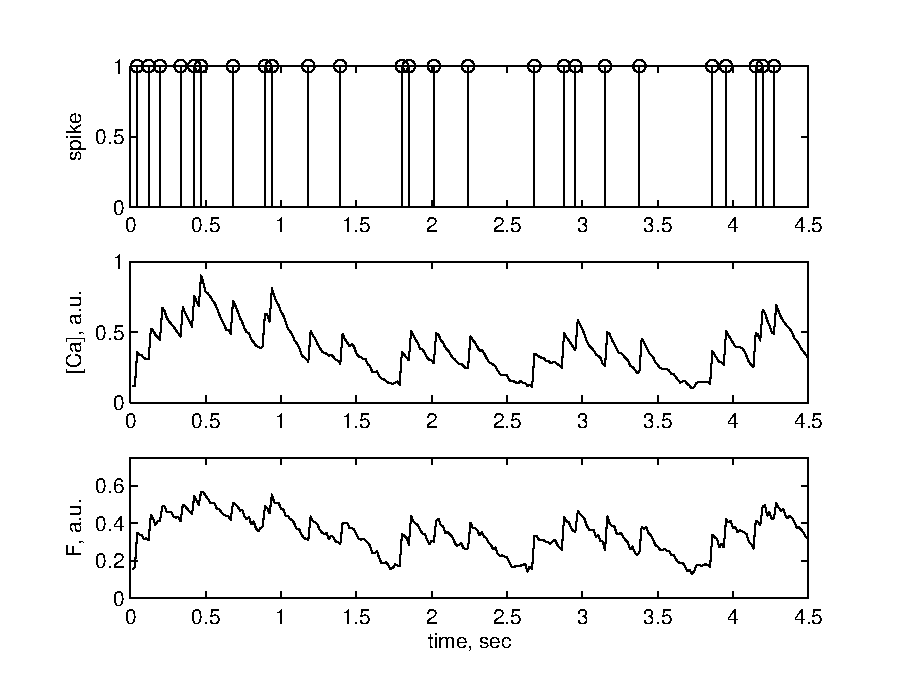
\includegraphics[width=\hsize]{../figs/Figure0a_fluor_eg_highSNR}
\end{minipage}
\caption{Examples of calcium and fluorescence traces for low (photon budget 5 Kph/neuron/frame, left)
and high SNR regimes (photon budget 40 Kph/neuron/frame, right). XXX J will modify to have real data. XXX}
\label{fig:egfluor}
\end{figure}


\subsection{Inference of the functional connectivity from the simulated calcium imaging data}
\label{sec:results:inference}
\input{results_Inference.tex}

\section{Discussion}
\label{sec:discussion}
\paragraph{j's outline of discussion}

\begin{itemize}
\item summary of main point: using sparse prior, we can recover a large fraction of variance of connection weights, assuming reasonable SNR, parameters, and imaging rate.

\item $h_j$ vs. $h_{ij}$ reduces dimensionality of hidden space to $O(N)$ vs. $O(N^2)$, leading to our approach scaling well as $N \rightarrow$ big

\item $P(A|BC)\neq P(A|B)P(A|C)$ unless $B$ and $C$ are uncorrelated.  we use this property, correlation coefficient doesn't, cross-correlations, etc., do not.

\item for the same reason, hidden neurons might be a problem for us.  faster imaging, etc., should help alleviate that.

\item we can measure uncertainty in estimates, and use photo-stimulation to activate/deactivate small groups of neurons efficiently to help reduce variance in uncertainty.

\item certainly the issue of common input and unobserved neurons should be addressed a bit more in the discussion.  

\item we can also talk a bit more about future directions involving fully-bayesian inference of the parameters (ie, MCMC over the parameter space, not just over the hidden variables X) instead of the MAP approach we took here; i tried to set this up a bit in the methods.  

\item other important future work to mention: real data, faster mcmc sampling methods, dealing with nonstationarities (e.g. bleaching).

\item comparison with other work (e.g., duane's, Garofalo, Vakorina, transfer entropy, granger causality, etc.)
\end{itemize}

% \paragraph{y's mini-discussion}
% 
% Functional connectivity may fail to faithfully represent anatomical circuit structure if false correlations are present between different neurons, induced e.g. by common inputs, or if the dynamics of neural population is entirely concentrated on a low-dimensional subspace of the full configurational space ${\bf n}$. Note that these two statements are, in a sense, stating the same condition: if activity of different neurons is tightly correlated, their dynamics is concentrated on a low-dimensional plane and vice-versa - concentration of dynamics onto a low-dimensional plane will be perceived as correlation in activity of different neurons. In turn, low dimensionality of the neural dynamics may be caused by different factors, including common input, small subset of command neurons driving the circuit, or even emergent property of a network. Low dimensionality of neural dynamics results in that the inference problem becomes underdetermined, i.e. there may exist directions in ${\bf w}_i$ along which connectivity is not constrained by neural activity data (i.e. directions orthogonal to the subspace of all observed neural activity configurations), or is poorly constrained. This, naturally, leads to ${\bf w}_i$ being poorly defined along these directions. The necessary condition for good correspondence between functional connectivity weights ${\bf w}_i$ and anatomical connectivity, therefore, is {\em full-dimensionality} of the observed set of neural configurations. In case of spontaneously firing system of neurons this condition is satisfied by many neuron-firings occurring independently, thus, allowing to fully sample all possible directions in ${\bf w}_i$.  Still, spontaneously active preparation by itself may fail to display sufficient degree of independence between firing of neurons due to low-dimensionality of observed activity space, e.g. because of emergent properties of the circuit. In that case necessary variety of independent neural activity patterns may be enforced by randomly activating subsets of neurons via ChR2 or glutamate uncaging.
% 
% We also note that the correlations induced by secondary and so on synaptic transmissions (such as when neuron $A$ results in firing of neuron $B$, which in turn results in firing by neuron $C$), are all properly resolved in GLM-fitting process via the so called explaining-away process. In other words, because we do not just identify correlations between neural firings with the functional connectivity weights $\w_{ij}$, but instead statistically fit a model of neural interactions, if found weights between neurons $A$ and $B$, and $B$ and $C$ are sufficient to explain the correlation between $A$ and $C$, the weight connecting $A$ and $C$ will not appear in the model - the correlation between $A$ and $C$ was ``explained away'' by correlations between $A$ and $B$, and $B$ and $C$. By this, the multi-synaptic firing patterns do not confuse our estimation process.
% 
% ADD SOME RAVINGS ABOUT PROPER/IMPROPER FUNCTIONAL CONNECTIVITY.


\begin{acknowledgments}
% \section*{Acknowledgements}
Thank everyone for their help and support [Bows, Bows, Bows] !!!
\end{acknowledgments}

\bibliography{mybib}
\bibliographystyle{amsplain}

\end{document}
